\graphicspath{{./chapters/chapter1/}}
\chapter{ }

% \section{Extension of the Two-Rounds Algorithm}
% \label{chap1-sec:modified_two_rounds}
% aaa

% \section{Basic Notations}
% \label{chap1-sec:notations}

% Table~\ref{chap1-tab:notations} shows the basic notations used in this paper.

\section{Effectiveness of empirical estimation in \alg{LocalRR$_\triangle$}}
\label{chap1-sec:RR_emp}
In Section~\ref{chap1-sub:non-interactive_triangles}, we presented \alg{LocalRR$_\triangle$}, which uses the empirical estimation method after the RR. 
Here we show the effectiveness of empirical estimation by comparing \alg{LocalRR$_\triangle$} with the RR without empirical estimation \cite{Qin_CCS17,Ye_ICDE20}. 
% i.e., the randomized neighbor list in \cite{Qin_CCS17}. 
% This method was also used in \cite{Ye_ICDE20}. 
% We also note that the RR has been applied to the adjacency matrix without empirical estimation in \cite{Qin_CCS17,Ye_ICDE20} for different purposes than counting triangles. 

As the RR without empirical estimation, we applied the RR to the lower triangular part of the adjacency matrix $\bmA$; i.e., we ran lines 1 to 6 in Algorithm~\ref{chap1-alg:subgraph-rr}. 
% This is the extended version of the randomized neighbor list \cite{Qin_CCS17}, as described in Section
Then we output the number of noisy triangles $m_3$. 
We denote this algorithm by \alg{RR w/o emp}. 
% Both \alg{LocalRR$_\triangle$} and \alg{RR w/o emp} provide $\epsilon$-edge LDP and $\epsilon$-entire edge LDP. 

% \begin{table}[t]
% \caption{Basic notations in this paper.} 
% \centering
% \hbox to\hsize{\hfil
% \begin{tabular}{l|l}
% \hline
% Symbol		&	Description\\
% \hline
% $n$         &	    Number of users.\\
% $G=(V,E)$   &	    Graph with $n$ nodes (users) $V$ and edges $E$.\\
% $v_i$       &       $i$-th user in $V$.\\
% $d_{max}$   &       Maximum degree of $G$.\\
% $\td_{max}$   &       Upper-bound on $d_{max}$ (used for projection).\\
% $\calG$     &       Set of possible graphs on $n$ users.\\
% $\bmA=(a_{i,j})$	    &		Adjacency matrix.\\
% $\bma_i$	&		$i$-th row of $\bmA$ (i.e., neighbor list of $v_i$).\\
% $\calR_i$     &       Randomized algorithm on $\bma_i$.\\
% $f_\triangle(G)$   &  Number of triangles in $G$.\\
% $f_{k\star}(G)$    &  Number of $k$-stars in $G$.\\
% \hline
% \end{tabular}
% \hfil}
% \label{chap1-tab:notations}
% \end{table}

Figure~\ref{chap1-fig:res5_RR_wo_emp} shows the $l_2$ loss of \alg{LocalRR$_\triangle$} and \alg{RR w/o emp} when we changed $n$ from $1000$ to $10000$ or $\epsilon$ in edge LDP from $0.1$ to $2$. 
The experimental set-up is the same as Section~\ref{chap1-sub:setup}. 
Figure~\ref{chap1-fig:res5_RR_wo_emp} shows that \alg{LocalRR$_\triangle$} significantly outperforms \alg{RR w/o emp}, which means that the $l_2$ loss is significantly reduced by empirical estimation. 
As shown in Section~\ref{chap1-sec:experiments}, the $l_2$ loss of \alg{LocalRR$_\triangle$} is also significantly reduced by an additional round of interaction.

\begin{figure}[t]
\centering
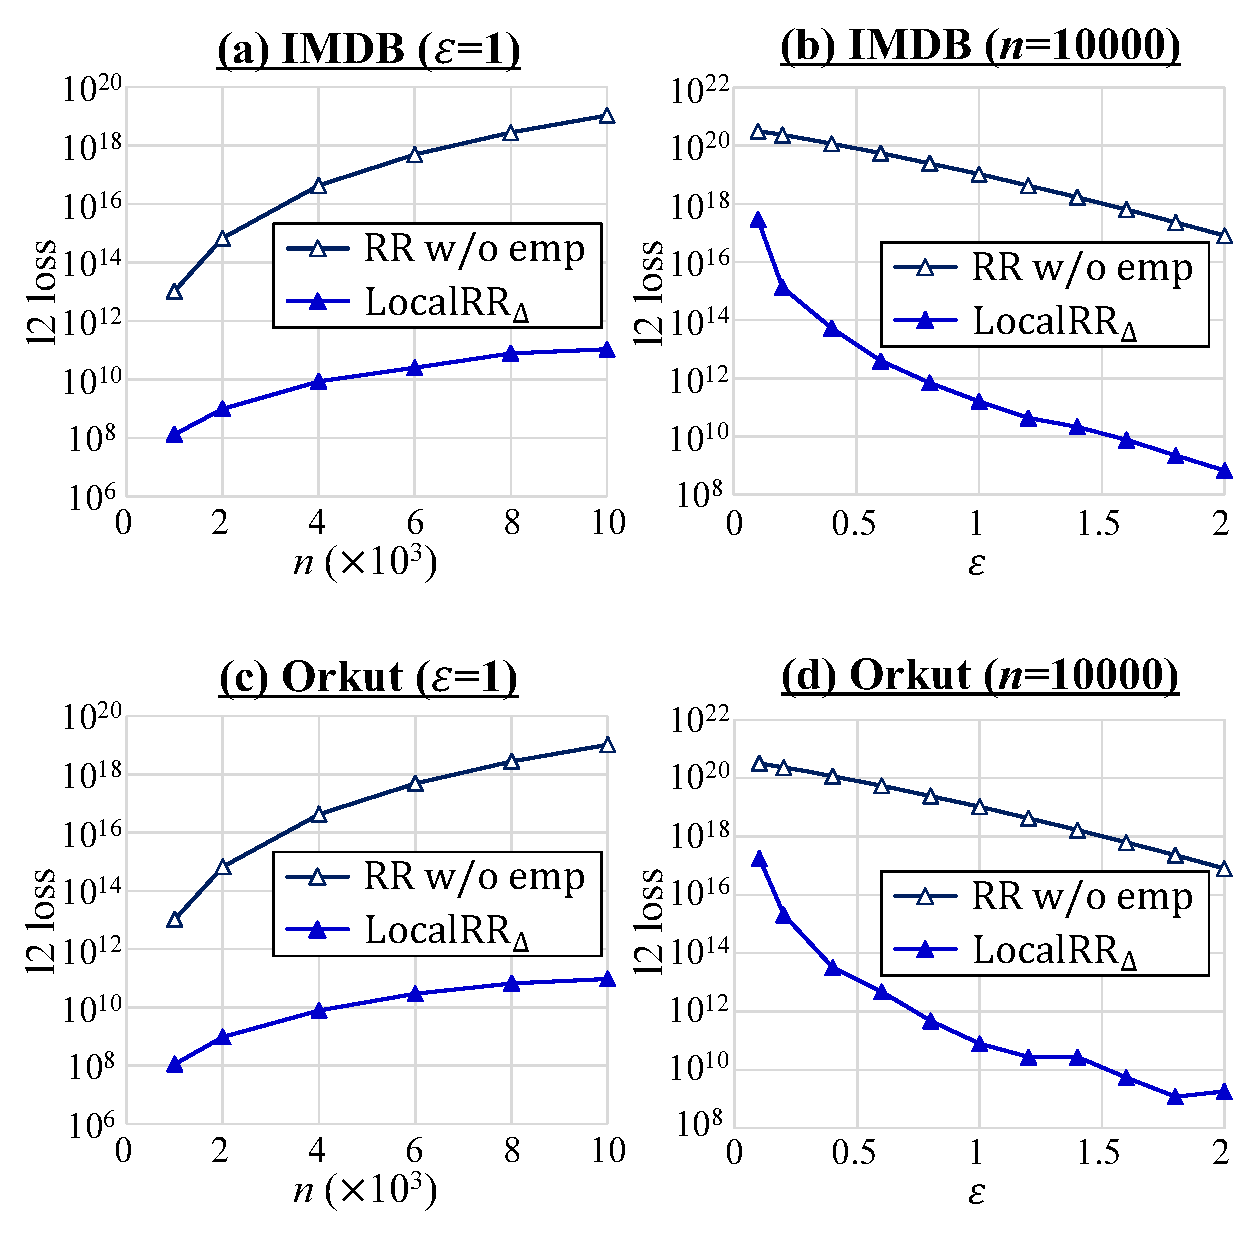
\includegraphics[width=0.99\linewidth]{fig/res5_RR_wo_emp.pdf}
\vspace{-5mm}
\caption{$l_2$ loss of \alg{LocalRR$_\triangle$} and the RR without empirical estimation (\alg{RR w/o emp}).}
\label{chap1-fig:res5_RR_wo_emp}
\end{figure}

\section{Experiments on Barab\'{a}si-Albert Graphs}
\label{chap1-sec:BAGraph}
% \smallskip
\noindent{\textbf{Experimental set-up.}}~~In Section~\ref{chap1-sec:experiments}, we evaluated our algorithms using two real datasets: \IMDB{} and \Orkut{}. 
We also evaluated our algorithms using artificial graphs that have power-law degree distributions. 
% based on 
We used the BA (Barab\'{a}si-Albert) model \cite{NetworkScience} to generate such graphs.

In the BA model, an artificial graph (referred to as a BA graph)
% of $n$ nodes 
is grown by adding new nodes one at a time. 
Each new node is connected to $\lambda \in \nats$ existing nodes with probability proportional to the degree of the existing node. 
% the number of edges that the existing nodes have. 
In our experiments, we used 
NetworkX \cite{Hagberg_SciPy08}, a Python package for graph analysis, to generate BA graphs.

We generated a BA graph $G^*$ with $1000000$ nodes using NetworkX. 
For the attachment parameter $\lambda$, we set $\lambda=10$ or $50$. 
When $\lambda=10$ (resp.~$50$), the average degree of $G^*$ was $10.0$ (resp.~$50.0$). 
For each case, we randomly generated $n$ users from the whole graph $G^*$, and extracted a graph $G=(V,E)$ with the $n$ users. 
Then we estimated the number of triangles $f_\triangle(G)$ and the number of $2$-stars $f_{2\star}(G)$. 
For triangles, we evaluated \alg{LocalRR$_\triangle$}, \alg{Local2Rounds$_\triangle$}, and \alg{CentralLap$\triangle$}. 
For $2$-stars, we evaluated \alg{LocalLap$_2\star$} and \alg{CentralLap$_2\star$}. 
In \alg{Local2Rounds$_\triangle$}, we set $\epsilon_1 = \epsilon_2$.
For $\td_{max}$, we set $\td_{max} = d_{max}$. 

We evaluated the $l_2$ loss while changing $n$ and $\epsilon$. 
We attempted $\gamma \in \nats$ ways to randomly select $n$ users from $G^*$, and averaged the $l_2$ loss over all the $\gamma$ ways to randomly select $n$ users. 
As with Section~\ref{chap1-sec:experiments}, we set $\gamma=100$ and changed $n$ from $1000$ to $10000$ while fixing $\epsilon=1$. 
Then we set $\gamma=10$ and changed $\epsilon$ from $0.1$ to $2$ while fixing $n=10000$.
% When we changed $n$ from $1000$ to $10000$ while fixing $\epsilon=1$, we set $\gamma = 100$. 
% When we changed $\epsilon$ from $0.1$ to $2$ while fixing $n=10000$, we set $\gamma = 10$.

\smallskip
\noindent{\textbf{Experimental results.}}~~Figure~\ref{chap1-fig:res6_BAGraph} shows the results. 
Overall, Figure~\ref{chap1-fig:res6_BAGraph} has a similar tendency to Figures~\ref{chap1-fig:res1_n_l2loss_tri}, \ref{chap1-fig:res1_n_l2loss_kst}, and \ref{chap1-fig:res2_eps_l2loss}. 
For example, \alg{Local2Rounds$_\triangle$} significantly outperforms \alg{LocalRR$_\triangle$}, especially when the graph $G$ is sparse; i.e., $\lambda = 10$. 
In \alg{Local2Rounds$_\triangle$}, \alg{CentralLap$\triangle$}, \alg{LocalLap$_2\star$}, and \alg{CentralLap$_2\star$}, the $l_2$ loss increases with increase in $\lambda$. 
This is because the maximum degree $d_{max}$ $(= \td_{max})$ increases with increase in $\lambda$.

\begin{figure}[t]
\centering
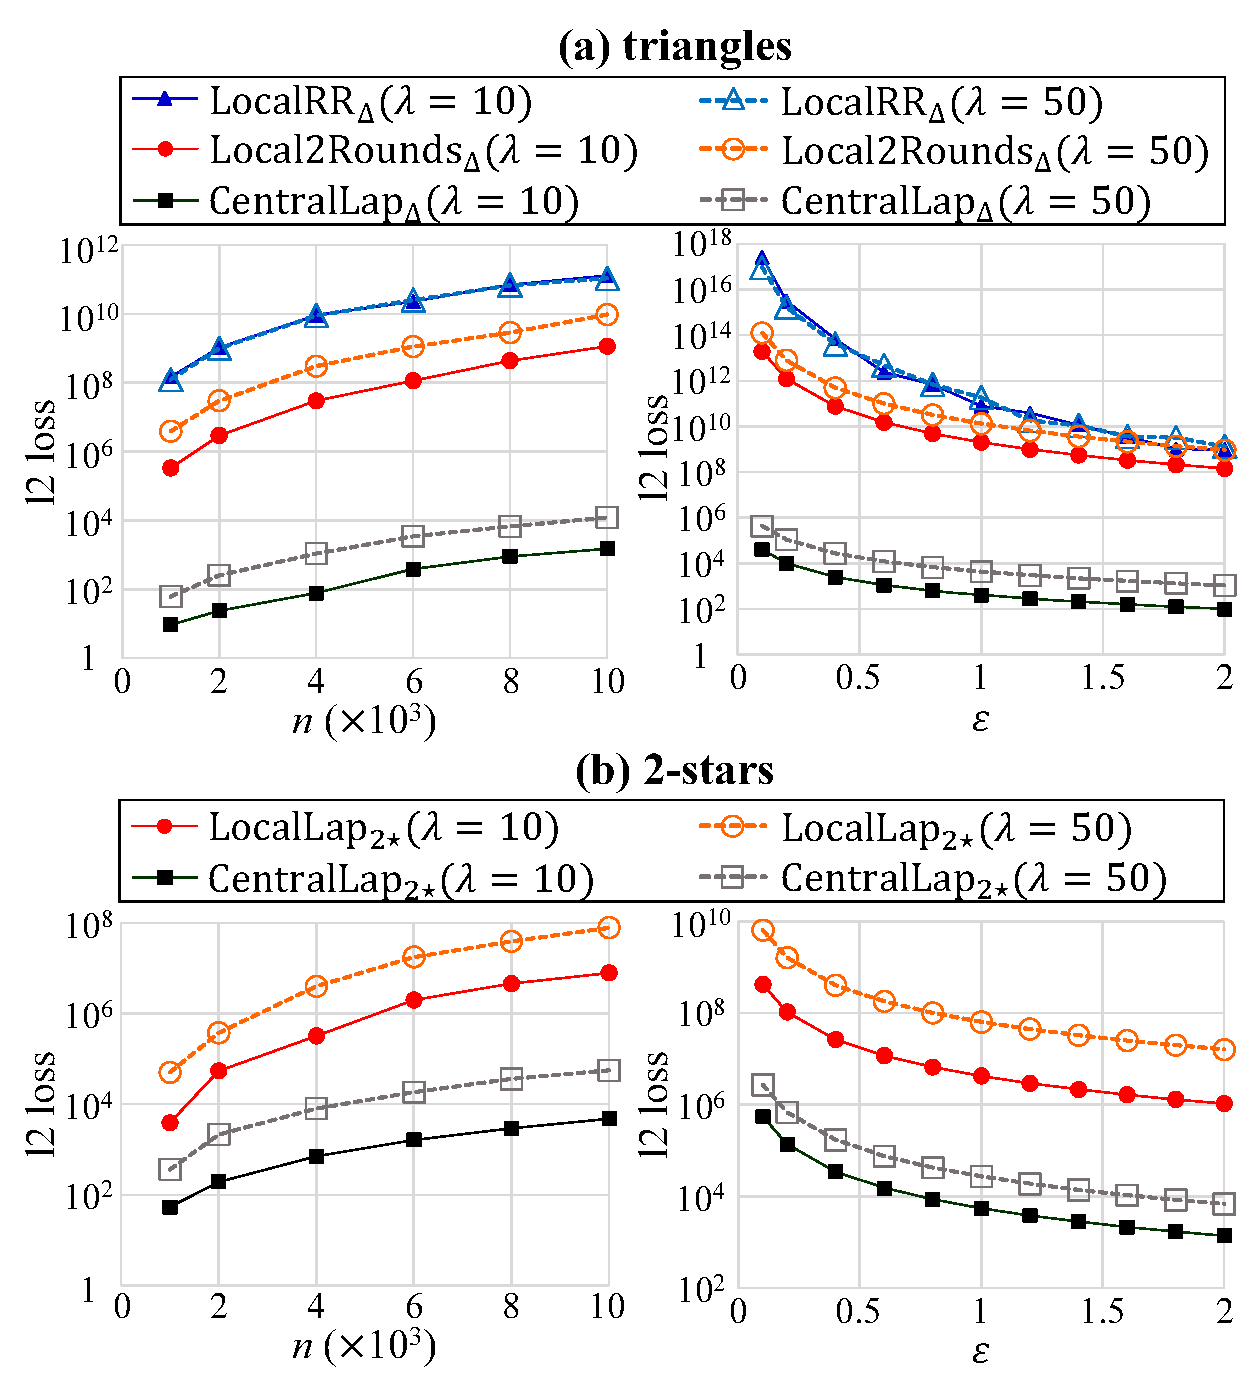
\includegraphics[width=0.99\linewidth]{fig/res6_BAGraph.pdf}
\vspace{-2mm}
\caption{$l_2$ loss in the Barab\'{a}si-Albert graph datasets 
% We set $\epsilon=1$ ($\epsilon_1 = \epsilon_2 = \frac{1}{2}$) in the left figures, and $n=10000$ in the right figures. 
(left: $\epsilon=1$, right: $n=10000$). 
We set the attachment parameter $\lambda$ in the BA model to $\lambda=10$ or $50$, and $\td_{max}$ to $\td_{max} = d_{max}$.}
\label{chap1-fig:res6_BAGraph}
\end{figure}

Figure~\ref{chap1-fig:res6_BAGraph} also shows that the $l_2$ loss is roughly consistent with our upper-bounds in Section~\ref{chap1-sec:algorithms}. 
For example, recall that \alg{LocalRR$_\triangle$}, \alg{Local2Rounds$_\triangle$}, \alg{CentralLap$_\triangle$}, \alg{LocalLap$_{2\star}$}, and \alg{CentralLap$_{2\star}$} achieve the expected $l_2$ loss of $O(n^4)$, $O(nd_{max}^3)$, $O(d_{max}^2)$, $O(nd_{max}^{2})$, and $O(d_{max}^{2})$, respectively. 
Assuming that $d_{max} = O(n)$, the left panels of Figure~\ref{chap1-fig:res6_BAGraph} are roughly consistent with these upper-bounds. 
In addition, the right panels of Figure~\ref{chap1-fig:res6_BAGraph} show that when we set $\lambda=10$ and decrease $\epsilon$ from $0.4$ to $0.1$, the $l_2$ loss increases by a factor of about $3800$, $250$, and $16$ in \alg{LocalRR$_\triangle$}, \alg{Local2Rounds$_\triangle$}, and \alg{CentralLap$_\triangle$}, respectively. 
They are roughly consistent with our upper-bounds -- for small $\epsilon$, the expected $l_2$ loss of \alg{LocalRR$_\triangle$}, \alg{Local2Rounds$_\triangle$}, and \alg{CentralLap$_\triangle$} is  $O(\epsilon^{-6})$, $O(\epsilon^{-4})$, and $O(\epsilon^{-2})$, respectively.

In summary, for both the two real datasets and the BA graphs, our experimental results showed the following findings: 
(1) \alg{Local2Rounds$_\triangle$} significantly outperforms \alg{LocalRR$_\triangle$}, especially when the graph $G$ is sparse; 
(2) our experimental results are roughly consistent with our upper-bounds.

% \subsection{Construction of an $(n, \frac{d_{max}}{2}-2)$ independent cube for $f_\triangle$}
\section{Construction of an $(n, \frac{d_{max}}{2}-2)$ independent cube for $f_\triangle$}
\label{chap1-sub:cube_triangle}
Suppose that $n$ is even and $d_{max}$ is divisible by $4$.
Since $d_{max} < n$, it is possible to write 
% $n = k \frac{d_{max}}{2} + r$ 
$n = \eta_1 \frac{d_{max}}{2} + \eta_2$ 
for integers 
% $k,r$ 
$\eta_1, \eta_2$
such that 
% $k \geq 1$ and $1 \leq r < \frac{d_{max}}{2}$. 
$\eta_1 \geq 1$ and $1 \leq \eta_2 < \frac{d_{max}}{2}$. 
Because 
% $k \frac{d_{max}}{2}$ 
$\eta_1 \frac{d_{max}}{2}$ 
and $n$ are even, 
we must have 
% $r$ 
$\eta_2$ 
is even.
Now, we can write 
% $n = (k-1) \frac{d_{max}}{2} + (r+\frac{d_{max}}{2})$.
$n = (\eta_1-1) \frac{d_{max}}{2} + (\eta_2 + \frac{d_{max}}{2})$.
% This means 
Thus, 
we can define 
% the 
a graph $G=(V,E)$ on $n$ 
% vertices 
nodes 
consisting of 
% $(k-1)$ 
$(\eta_1-1)$ 
cliques of 
even 
size
$\frac{d_{max}}{2}$ and one final clique of an even size $\eta_2+\frac{d_{max}}{2} \in (\frac{d_{max}}{2}, d_{max})$ 
% between $\frac{d_{max}}{2}$ and $d_{max}$ 
with all cliques disjoint. 

Since $G=(V,E)$ consists of even-sized cliques, it contains a perfect matching $M$. 
Figure~\ref{chap1-fig:mono-cube_triangle} shows examples of $G$ and $M$, where $n=14$, $d_{max} = 8$, $\eta_1 = 3$, and $\eta_2 = 2$. 
Let 
% $G' = G \setminus M$. 
$G'=(V,E')$ such that $E' = E \setminus M$. 
Let $\calA = \{(V,E' \cup N: N \subseteq M\}$. 
Each edge in $G$ is part of at least $\frac{d_{max}}{2}-2$ triangles. 
For each pair of edges in $M$, the triangles of $G$ of which they are part
are disjoint. 
Thus, 
% for any $N \subseteq M$, with $e \in N$, 
for any edge $e \in M$, 
removing $e$ 
% $e \in N$
from 
% $G \setminus N$ 
a graph in $\calA$ 
will remove at least $\frac{d_{max}}{2}-2$ triangles. This implies 
that $\calA$ 
% $\calA = \{G \cup N : N \subseteq M\}$ 
is an $(n,\frac{d_{max}}{2}-2)$ independent cube for $f_\triangle$.

%Similarly, for even natural number $l \in \nats$ such that $d_{max}>l+2$, we can construct an $(n,d_{max}-l-2)$ independent cube from the adjacency matrix of a collection of cliques of size $d_{max}-l$.

\begin{figure}[t]
  \centering
  %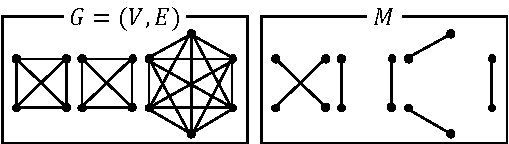
\includegraphics[width=0.88\linewidth]{fig/MonoCube_triangle.pdf}
  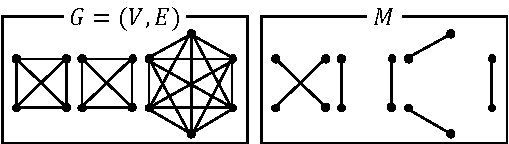
\includegraphics[width=0.88\linewidth]{fig/IndCube_triangle.pdf}
  \vspace{-2mm}
  \caption{
    Examples of $G$ and $M$ for constructing an independent cube for $f_\triangle$ ($n=14$, $d_{max} = 8$, $\eta_1 = 3$, $\eta_2 = 2$).
  }\label{chap1-fig:mono-cube_triangle}
\end{figure}


\arxiv{
\section{Proof of Statements in Section~\ref{chap1-sec:algorithms}}
\label{chap1-sec:proof}
Here we prove the statements in Section~\ref{chap1-sec:algorithms}. 
Our proofs will repeatedly use the well-known bias-variance decomposition \cite{mlpp}, which we briefly explain below. 
We denote the variance of the random variable $X$ by $\mathbb{V}[X]$. 
If we are producing a private, randomized estimate $\hat{f}(G)$ of the graph function $f(G)$, then the expected $l_2$ loss (over the randomness in the algorithm) can be written as: 
\begin{equation}\label{chap1-eq:bias-var}
  \E[l_2^2(\hat{f}(G),f(G))] = \left(\E[\hat{f}(G)] - f(G)\right)^2
  + \V[\hat{f}(G)].
\end{equation}
The first term is the bias, and the second term is the variance. 
If the estimate is unbiased (i.e., $\E[\hat{f}(G)] = f(G)$), then the expected $l_2$ loss is equal to the variance.

\subsection{Proof of Theorem~\ref{chap1-thm:k-stars_LDP}}
Let $\calR_i$ be \alg{LocalLap$_{k\star}$}. 
Let $d_i,d'_i \in \nnints$ be the number of ``1''s in two neighbor lists $\bma_i,\bma'_i \in \{0,1\}^n$ that differ in one bit. 
% Consider two neighbor lists $\bma_i,\bma'_i \in \{0,1\}^n$ that differ in one bit. 
% Let $d_i$ (resp.~$d'_i$) $\in \nnints$ be the number of ``1''s in $\bma_i$ (resp.~$\bma'_i$). 
Let $r_i = \binom{d_i}{k}$ and $r'_i = \binom{d'_i}{k}$. 
Below we consider two cases about $d_i$: when $d_i < \td_{max}$ and when $d_i \geq \td_{max}$.

\smallskip
\noindent{\textbf{Case 1: $d_i < \td_{max}$.}}~~In this case, both $\bma_i$ and $\bma'_i$ do not change after graph projection, as $d'_i \leq d_i + 1 \leq \td_{max}$. 
Then we obtain:
\begin{align*}
\Pr[\calR_i(\bma_i) = \hr_i] &= \exp\left(-\frac{\epsilon |\hr_i- r_i|}{\Delta}\right) \\
\Pr[\calR_i(\bma'_i) = \hr_i] &= \exp\left(-\frac{\epsilon |\hr_i- r'_i|}{\Delta}\right),
\end{align*}
where $\Delta = \binom{\td_{max}}{k-1}$. 
Therefore, 
% and hence 
\begin{align}
\frac{\Pr[\calR_i(\bma_i) = \hr_i]}{\Pr[\calR_i(\bma'_i) = \hr_i]} 
&= \exp\left( \frac{\epsilon |\hr_i- r'_i|}{\Delta} - \frac{\epsilon |\hr_i- r_i|}{\Delta}\right) \nonumber\\
&\leq  \exp\left( \frac{\epsilon |r'_i- r_i|}{\Delta} \right) \label{chap1-eq:Pr_R_i_a'_i_a_i}\\
& \hspace{4mm} (\text{by the triangle inequality}). \nonumber
\end{align}
If $d'_i = d_i + 1$, then $|r'_i- r_i|$ in (\ref{chap1-eq:Pr_R_i_a'_i_a_i}) can be written as follows:
\begin{align*}
|r'_i- r_i| 
= \binom{d_i+1}{k} - \binom{d_i}{k} 
= \binom{d_i}{k-1}
< \binom{\td_{max}}{k-1}
= \Delta, 
\end{align*}
Since we add $\Lap(\frac{\Delta}{\epsilon})$ to $r_i$, we obtain:
\begin{align}
\Pr[\calR_i(\bma_i) = \hr_i] \leq e^\epsilon \Pr[\calR_i(\bma'_i) = \hr_i]. 
\label{chap1-eq:R_i_a_i_hr_i}
\end{align}
If $d'_i = d_i - 1$, then $|r'_i- r_i| = \binom{d_i}{k} - \binom{d_i-1}{k} = \binom{d_i-1}{k-1} < \Delta$ and (\ref{chap1-eq:R_i_a_i_hr_i}) holds. 
Therefore, \alg{LocalLap$_{k\star}$} provides $\epsilon$-edge LDP. 

\smallskip
\noindent{\textbf{Case 2: $d_i \geq \td_{max}$.}}~~Assume 
% Second, we consider the case where $d_i \geq \td_{max}$. 
that $d'_i = d_i + 1$. 
In this case, $d'_i > \td_{max}$. 
Therefore, $d'_i$ becomes $\td_{max}$ after graph projection. 
In addition, 
% If $d_i > \td_{max}$, then 
$d_i$ also becomes $\td_{max}$ after graph projection. 
Therefore, we obtain 
$d_i = d'_i = \td_{max}$ after graph projection. 
Thus 
% and $r_i = r'_i = \binom{\td_{max}}{k}$. 
% Therefore, 
$\Pr[\calR_i(\bma_i) = \hr_i] = \Pr[\calR_i(\bma'_i) = \hr_i]$. 

Assume that $d'_i = d_i - 1$. 
If $d_i > \td_{max}$, then $d_i = d'_i = \td_{max}$ after graph projection. 
Thus $\Pr[\calR_i(\bma_i) = \hr_i] = \Pr[\calR_i(\bma'_i) = \hr_i]$. 
If $d_i = \td_{max}$, then (\ref{chap1-eq:R_i_a_i_hr_i}) holds. 
Therefore, \alg{LocalLap$_{k\star}$} provides $\epsilon$-edge LDP. \qed

\subsection{Proof of Theorem~\ref{chap1-thm:k-stars}}
Assuming the maximum degree $d_{max}$ of $G$ is at most $\td_{max}$, the only
randomness in the algorithm will be the Laplace noise since graph projection
will not occur.
Since the Laplacian noise $\Lap(\frac{\Delta}{\epsilon})$ has mean $0$, the estimate $\hf_{k\star}(G, \epsilon, \td_{max})$ is unbiased. 
Then by the bias-variance decomposition \cite{mlpp}, 
the expected $l_2$ loss 
$\mathbb{E}[l_2^2(\hf_{k\star}(G, \epsilon, \td_{max}),\allowbreak f_{k\star}(G))]$ is equal to the variance of $\hf_{k\star}(G, \epsilon, \td_{max})$. 
% We denote the variance of the random variable $X$ by $\mathbb{V}[X]$. 
The variance of $\hf_{k\star}(G, \epsilon, \td_{max})$ can be written as follows:
\begin{align*}
    \mathbb{V}[\hf_{k\star}(G, \epsilon, \td_{max})] 
    &= \mathbb{V}\left[ \sum_{i=1}^n \Lap\left( \frac{\Delta}{\epsilon} \right) \right] \\
    &= \frac{n \Delta^2}{\epsilon^2}.
\end{align*}
% Note that $\tilde{m}_3$ and $\tilde{m}_0$ are not dependent. 
Since $\Delta = \binom{\td_{max}}{k-1} = O(\td_{max}^{k-1})$, we obtain:
\begin{align*}
    \mathbb{E}[l_2^2(\hf_{k\star}(G, \epsilon, \td_{max}), f_{k\star}(G))] 
    &= \mathbb{V}[\hf_{k\star}(G, \epsilon, \td_{max})] \\
    &= O\left(\frac{n \td_{max}^{2k-2}}{\epsilon^2}\right).
\end{align*}
\qed

\subsection{Proof of Proposition~\ref{chap1-prop:triangle_emp}}
Let $\mu = e^\epsilon$ and $\bmQ \in [0,1]^{4 \times 4}$ be a $4 \times 4$ matrix such that:
\begin{align}
  \bmQ = \frac{1}{(\mu+1)^3} \left(
    \begin{array}{cccc}
      \mu^3 & 3\mu^2 & 3\mu & 1 \\
      \mu^2 & \mu^3+2\mu & 2\mu^2+1 & \mu \\
      \mu & 2\mu^2+1 & \mu^3+2\mu & \mu^2 \\
      1 & 3\mu & 3\mu^2 & \mu^3
    \end{array}
  \right).
  \label{chap1-eq:Q_1}
\end{align}
Let $c_3, c_2, c_1, c_0 \in \nnints$ be respectively the number of triangles, 2-edges, 1-edge, and no-edges in $G$. 
Then we obtain:
\begin{align}
(\mathbb{E}[m_3], \mathbb{E}[m_2], \mathbb{E}[m_1],
\mathbb{E}[m_0]) = (c_3, c_2, c_1, c_0) \bmQ.
\label{chap1-eq:bmQ}
\end{align}
In other words, $\bmQ$ is a transition matrix from a type of subgraph (i.e., triangle, 2-edges, 1-edge, or no-edge) in $G$ to a type of subgraph in $G'$. 

Let $\hat{c}_3, \hat{c}_2, \hat{c}_1, \hat{c}_0 \in \reals$ be the empirical estimate of $(c_3, c_2, c_1, c_0)$. 
By (\ref{chap1-eq:bmQ}), they can be written as follows:
\begin{align}
(\hat{c}_3, \hat{c}_2, \hat{c}_1, \hat{c}_0) = (m_3, m_2, m_1, m_0) \bmQ^{-1}.
\label{chap1-eq:hc3_hc2_hc1_hc0}
\end{align}
Let $\bmQ_{i,j}^{-1}$ be the ($i,j$)-th element of $\bmQ^{-1}$. 
By using Cramer's rule, we obtain: 
\begin{align}
\bmQ_{1,1}^{-1} &= \textstyle{\frac{\mu^3}{(\mu-1)^3}},~ \bmQ_{2,1}^{-1} =  \textstyle{-\frac{\mu^2}{(\mu-1)^3}}, \label{chap1-eq:bmQ11_bmQ21}\\
\bmQ_{3,1}^{-1} &= \textstyle{\frac{\mu}{(\mu-1)^3}},~ \bmQ_{4,1}^{-1} = \textstyle{-\frac{1}{(\mu-1)^3}}.
\label{chap1-eq:bmQ31_bmQ41}
\end{align}
By (\ref{chap1-eq:hc3_hc2_hc1_hc0}), (\ref{chap1-eq:bmQ11_bmQ21}), and (\ref{chap1-eq:bmQ31_bmQ41}), we obtain:
\begin{align*}
\textstyle{\hat{c}_3 = \frac{\mu^3}{(\mu-1)^3} m_3 - \frac{\mu^2}{(\mu-1)^3} m_2 + \frac{\mu}{(\mu-1)^3} m_1 - \frac{1}{(\mu-1)^3} m_0.}
\end{align*}
Since $\mu = e^\epsilon$ and the empirical estimate is unbiased \cite{Kairouz_ICML16,Wang_USENIX17}, we obtain (\ref{chap1-eq:triangle_emp}) in Proposition~\ref{chap1-prop:triangle_emp}. \qed

\subsection{Proof of Theorem~\ref{chap1-thm:subgraph-rr_LDP}}
Since \alg{LocalRR$_\triangle$} applies the RR to the lower triangular part of the adjacency matrix $\bmA$, it provides $\epsilon$-edge LDP for $(R_1, \ldots, R_n)$. 
Lines 5 to 8 in Algorithm~\ref{chap1-alg:subgraph-rr} are post-processing of $(R_1, \ldots, R_n)$. 
Thus, by the immunity to post-processing \cite{DP}, \alg{LocalRR$_\triangle$} provides $\epsilon$-edge LDP for the output $\frac{1}{(\mu-1)^3}(\mu^3 m_3 -\mu^2 m_2 + \mu m_1 - m_0)$. 

In addition, the existence of edge $(v_i,v_j) \in E$ $(i>j)$ affects only one element $a_{i,j}$ in the lower triangular part of $\bmA$. 
Therefore, \alg{LocalRR$_\triangle$} provides $\epsilon$-relationship DP.

\subsection{Proof of Theorem~\ref{chap1-thm:subgraph-rr}}
\label{chap1-sub:proof_thm:subgraph-rr}
By Proposition~\ref{chap1-prop:triangle_emp}, the estimate $\hf_{\triangle}(G, \epsilon)$ by \alg{LocalRR$_\triangle$} is unbiased. 
Then by the bias-variance decomposition \cite{mlpp}, 
the expected $l_2$ loss $\mathbb{E}[l_2^2(\hf_{\triangle}(G, \epsilon), f_\triangle(G))]$ is equal to the variance of $\hf_{\triangle}(G, \epsilon)$. 
% We denote the variance of the random variable $X$ by $\mathbb{V}[X]$. 
Let 
$a_3 = \frac{\mu^3}{(\mu-1)^3}$, 
$a_2 = - \frac{\mu^2}{(\mu-1)^3}$, 
$a_1 = \frac{\mu}{(\mu-1)^3}$, and 
$a_0 = - \frac{1}{(\mu-1)^3}$. 
Then the variance of $\hf_{\triangle}(G, \epsilon)$ can be written as follows:
\begin{align}
    \V[\hf_{\triangle}(G, \epsilon)] 
    &= \V[a_3 m_3 + a_2 m_2 + a_1 m_1 + a_0 m_0] \nonumber\\
    &= a_3^2 \V[m_3] + a_2^2 \V_{RR}[m_2] + a_1^2 \V[m_1] + a_0^2 \V[m_0] \nonumber\\
    &\hspace{3.5mm} + \sum_{i=0}^3 \sum_{j=0, j \ne i}^3 2a_i a_j \text{cov}(m_i, m_j),
    \label{chap1-eq:V_a3m3_a2m2_a1m1_a0m0}
\end{align}
where $\text{cov}(m_i, m_j)$ represents the covariance of $m_i$ and $m_j$. 
The covariance $\text{cov}(m_i, m_j)$ can be written as follows:
\begin{align}
    \text{cov}(m_i, m_j)
    &\leq \sqrt{\V[m_i] \V[m_j]} \nonumber\\
    &\hspace{4.2mm} (\text{by Cauchy-Schwarz inequality}) \nonumber\\
    &\leq  \max\{ \V[m_i], \V[m_j]\} \nonumber\\
    &\leq \V[m_i] + \V[m_j].
    \label{chap1-eq:cov_mi_mj}
\end{align}
By (\ref{chap1-eq:V_a3m3_a2m2_a1m1_a0m0}) and (\ref{chap1-eq:cov_mi_mj}), we obtain:
\begin{align}
    &\V[\hf_{\triangle}(G, \epsilon)] \nonumber\\
    &\leq (a_3^2 + 4a_3(a_2 + a_1 + a_0)) \V[m_3] \nonumber\\
    & \hspace{4.5mm} + (a_2^2 + 4a_2(a_3 + a_1 + a_0)) \V[m_2] \nonumber\\
    & \hspace{4.5mm} + (a_1^2 + 4a_1(a_3 + a_2 + a_0)) \V[m_1] \nonumber\\
    & \hspace{4.5mm} + (a_0^2 + 4a_0(a_3 + a_2 + a_1)) \V[m_0] \nonumber\\
    &= O\left( \frac{e^{6\epsilon}}{(e^\epsilon-1)^6} (\V[m_3] + \V[m_2] + \V[m_1] + \V[m_0]) \right).
    % &\leq O\left(\frac{e^{6\epsilon}}{(e^\epsilon-1)^6} \V[m_3] + \frac{e^{5\epsilon}}{(e^\epsilon-1)^6}\V[m_2]
    % \right. \nonumber\\
    % & \hspace{10mm} \left. + \frac{e^{4\epsilon}}{(e^\epsilon-1)^6}\V[m_1] + \frac{e^{3\epsilon}}{(e^\epsilon-1)^6}\V[m_0]\right).
    \label{chap1-V_RR_m_3}
\end{align}

Below we calculate $\V[m_3]$, $\V[m_2]$, $\V[m_1]$, and $\V[m_0]$ by assuming the Erd\"{o}s-R\'{e}nyi model $\bmG(n, \alpha)$ for $G$:

\begin{lemma}\label{chap1-lem:erdos-renyi-variance}
  Let $G \sim \textbf{G}(n,\alpha)$. 
  %with $\alpha < \frac{1}{2}$. 
  Let $p = \frac{1}{e^\epsilon+1}$ and 
  $\beta = \alpha(1-p) + (1-\alpha)p$. 
  Then $\V[m_3] = O(\beta^5 n^4 + \beta^3
  n^3)$, $\V[m_2] = O(\beta^3 n^4 + \beta^2 n^3)$, and 
  $\V[m_1] = \V[m_0] = O(\beta n^4)$.
\end{lemma}
% We prove Lemma~\ref{chap1-lem:erdos-renyi-variance} at the end of Appendix~\ref{chap1-sub:proof_thm:subgraph-rr}. 
Before going into the proof of Lemma~\ref{chap1-lem:erdos-renyi-variance}, we prove Theorem~\ref{chap1-thm:subgraph-rr} using Lemma~\ref{chap1-lem:erdos-renyi-variance}. 
By (\ref{chap1-V_RR_m_3}) and Lemma~\ref{chap1-lem:erdos-renyi-variance}, we obtain: 
\begin{align*}
\V[\hf_{\triangle}(G, \epsilon)] = O\left( \frac{e^{6\epsilon}}{(e^\epsilon-1)^6} \beta n^4 \right),
\end{align*}
which proves Theorem~\ref{chap1-thm:subgraph-rr}. \qed

We now prove Lemma~\ref{chap1-lem:erdos-renyi-variance}:

\begin{proof}[Proof of Lemma~\ref{chap1-lem:erdos-renyi-variance}]
Fist we show the variance of $m_3$ and $m_0$. 
Then we show the variance of $m_2$ and $m_1$.

\smallskip
\noindent{\textbf{Variance of $m_3$ and $m_0$.}}~~Since each edge in the original graph $G$ is independently generated with probability $\alpha \in [0,1]$, each edge in the noisy graph $G'$ is independently generated with probability $\beta = \alpha (1-p) + (1 - \alpha) p \in [0,1]$, where $p=\frac{1}{e^\epsilon+1}$. 
Thus $m_3$ is the number of triangles in graph $G' \sim \textbf{G}(n,\beta)$.

For $i,j,k \in [n]$, let $y_{i,j,k} \in \{0,1\}$ be a variable that takes $1$ if and only if 
$(v_i, v_j, v_k)$ forms a triangle. 
Then $\mathbb{E}[m_3^2]$ can be written as follows:
\begin{align}
  \mathbb{E}[m_3^2] = \sum_{i<j<k} ~ \sum_{i'<j'<k'}
  \mathbb{E}[y_{i,j,k} y_{i',j',k'}] 
  \label{chap1-eq:E_RR_tm3}
\end{align}
$\mathbb{E}[y_{i,j,k} y_{i',j',k'}]$ in (\ref{chap1-eq:E_RR_tm3}) is the probability that both $(v_i,v_j,v_k)$ and $(v_{i'},v_{j'},v_{k'})$ form a triangle. 
This event can be divided into the following four types:
\begin{enumerate}
\item $(i,j,k)=(i',j',k')$. There are $\binom{n}{3}$ such terms in (\ref{chap1-eq:E_RR_tm3}). 
For each term, $\mathbb{E}[y_{i,j,k} y_{i',j',k'}] = \beta^3$.
\item $(i,j,k)$ and $(i',j',k')$ have two elements in common. 
There are $\binom{n}{2} (n-2) (n-3) = 12\binom{n}{4}$ such terms in (\ref{chap1-eq:E_RR_tm3}). 
For each term, $\mathbb{E}[y_{i,j,k} y_{i',j',k'}] = \beta^5$. 
\item $(i,j,k)$ and $(i',j',k')$ have one element in common. 
There are $n \binom{n-1}{2} \binom{n-3}{2} = 30\binom{n}{5}$ such terms in (\ref{chap1-eq:E_RR_tm3}). 
For each term, $\mathbb{E}[y_{i,j,k} y_{i',j',k'}] = \beta^6$. 
\item $(i,j,k)$ and $(i',j',k')$ have no common elements. 
There are $\binom{n}{3} \binom{n-3}{3} = 20\binom{n}{6}$ such terms in in (\ref{chap1-eq:E_RR_tm3}). 
For each term, $\mathbb{E}[y_{i,j,k} y_{i',j',k'}] = \beta^6$. 
\end{enumerate}
Moreover, $\mathbb{E}[m_3]^2 = \binom{n}{3}^2 \beta^6$. 
Therefore, the variance of $m_3$ can be written as follows:
\begin{align*}
    \V[m_3] 
    &= \textstyle{\binom{n}{3} \beta^3 + 12\binom{n}{4} \beta^5 + 30\binom{n}{5} \beta^6 + 20\binom{n}{6} \beta^6 - \binom{n}{3}^2 \beta^6} \\
    &= \textstyle{\binom{n}{3} \beta^3 (1-\beta^3) + 12\binom{n}{4}\beta^5(1-\beta)} \\
    &= O(\beta^5 n^4 + \beta^3 n^3).
\end{align*}

By changing $\beta$ to $1-\beta$ and counting triangles, we get a random variable with the same distribution as $m_0$. Thus,
\begin{align*}
  \V[m_0] 
  &= \textstyle{\binom{n}{3} (1-\beta)^3(1-(1-\beta)^3) + 12\binom{n}{4} (1-\beta)^5\beta}
  \\
  &= O(\beta n^4).
\end{align*}
\smallskip
\noindent{\textbf{Variance of $m_2$ and $m_1$.}}~~For $i,j,k \in [n]$, let $z_{i,j,k} \in \{0,1\}$ be a variable that takes $1$ if and only if 
$(v_i, v_j, v_k)$ forms $2$-edges (i.e., exactly one edge is missing in the three nodes). 
Then $\mathbb{E}[m_2^2]$ can be written as follows:
\begin{align}
  \mathbb{E}[m_2^2] = \sum_{i<j<k} \sum_{i'<j'<k'}
  \mathbb{E}[z_{i,j,k} z_{i',j',k'}] 
  \label{chap1-eq:E_RR_tm2}
\end{align}
$\mathbb{E}[z_{i,j,k} z_{i',j',k'}]$ in (\ref{chap1-eq:E_RR_tm2}) is the probability that both $(v_i,v_j,v_k)$ and $(v_{i'},v_{j'},v_{k'})$ form $2$-edges. 
This event can be divided into the following four types:
\begin{enumerate}
	\item $(i,j,k)=(i',j',k')$. There are $\binom{n}{3}$ such terms in (\ref{chap1-eq:E_RR_tm2}). 
    For each term, $\mathbb{E}[z_{i,j,k} z_{i',j',k'}]=3\beta^2(1-\beta)$. 
	\item $(i,j,k)$ and $(i',j',k')$ have two elements in common. 
	There are $\binom{n}{2}(n-2)(n-3) = 12 \binom{n}{4}$ such terms in (\ref{chap1-eq:E_RR_tm2}). 
	For example, consider a term in which $i=i'=1$, $j=j'=2$, $k=3$, and $k'=4$. 
	Both $(v_1,v_2,v_3)$ and $(v_1,v_2,v_4)$ form 2-edges if:\\
	(a) $(v_1,v_2), (v_1,v_3), (v_1,v_4) \in E'$, $(v_2,v_3), (v_2,v_4) \notin E'$, \\
	(b) $(v_1,v_2), (v_1,v_3), (v_2,v_4) \in E'$, $(v_2,v_3), (v_1,v_4) \notin E'$, \\
	(c) $(v_1,v_2), (v_2,v_3), (v_1,v_4) \in E'$, $(v_1,v_3), (v_2,v_4) \notin E'$, \\
	(d) $(v_1,v_2), (v_2,v_3), (v_2,v_4) \in E'$, $(v_1,v_3), (v_1,v_4) \notin E'$, or \\
	(e) $(v_1,v_3), (v_1,v_4), (v_2,v_3), (v_2,v_4) \in E'$, $(v_1,v_2) \notin E'$. \\
    Thus, $\mathbb{E}[z_{i,j,k} z_{i',j',k'}]=4\beta^3(1-\beta)^2 + \beta^4(1-\beta)$ for this term. 
    Similarly, $\mathbb{E}[z_{i,j,k} z_{i',j',k'}]=4\beta^3(1-\beta)^2 + \beta^4(1-\beta)$ for the other terms.
	\item $(i,j,k)$ and $(i',j',k')$ have one element in common. 
	There are $n \binom{n-1}{2} \binom{n-3}{2} = 30\binom{n}{5}$ such terms in (\ref{chap1-eq:E_RR_tm2}).  For each term, $\mathbb{E}[z_{i,j,k}z_{i',j',k'}]=(3\beta^2(1-\beta))^2 = 9\beta^4(1-\beta)^2$. 
	\item $(i,j,k)$ and $(i',j',k')$ have no common elements. 
	There are $\binom{n}{3}\binom{n-3}{3} = 20\binom{n}{6}$ such terms in (\ref{chap1-eq:E_RR_tm2}). 
	For each term, $\mathbb{E}[z_{i,j,k}z_{i',j',k'}]=(3\beta^2(1-\beta))^2 = 9\beta^4(1-\beta)^2$. 
\end{enumerate}
Moreover, $\mathbb{E}[m_2]^2 = (3\binom{n}{3}\beta^2(1-\beta))^2 = 9\binom{n}{3}^2\beta^4(1-\beta)^2$. 
Therefore, the variance of $m_2$ can be written as follows:
\begin{align*}
  \mathbb{V}[m_2] 
  &= \mathbb{E}[m_2^2] - \mathbb{E}[m_2]^2 \nonumber\\
  &= \textstyle{3\binom{n}{3}\beta^2(1-\beta) + 12\binom{n}{4}\left(4\beta^3(1-\beta)^2 + \beta^4(1-\beta)\right)} \nonumber\\
  &\hspace{3.5mm} \textstyle{+ 270\binom{n}{5}\beta^4(1-\beta)^2 + 180\binom{n}{6}\beta^4(1-\beta)^2} \nonumber\\
  &\hspace{3.5mm} \textstyle{- 9\binom{n}{3}^2\beta^4(1-\beta)^2.}
\end{align*}
By simple calculations,
\begin{align*}
\textstyle{270\binom{n}{5} + 180\binom{n}{6} - 9\binom{n}{3}^2 = -108\binom{n}{4}-9\binom{n}{3}.}
\end{align*}
Thus we obtain:
\begin{align*}
\mathbb{V}[m_2] 
&= \textstyle{3\binom{n}{3}\beta^2(1-\beta)\left(1 - 3\beta^2(1-\beta)\right)} \nonumber\\
%&\hspace{3.5mm} \textstyle{+ 12\binom{n}{4}\left(4\beta^3(1-\beta)^2 + \beta^4(1-\beta) - 9\beta(1-\beta) \right)} \\
&\hspace{3.5mm} \textstyle{+ 12\binom{n}{4} \beta^3(1-\beta) \left(4(1-\beta) + \beta - 9\beta(1-\beta) \right)} \\
&= O(\beta^3 n^4 + \beta^2n^3).
\end{align*}
Similarly, the variance of $m_1$ can be written as follows:
\begin{align*}
\mathbb{V}[m_1] 
&= \textstyle{3\binom{n}{3}\beta(1-\beta)^2\left(1 - 3\beta(1-\beta)^2\right)} \nonumber\\
&\hspace{3.5mm} \textstyle{+ 12\binom{n}{4} \beta(1-\beta)^3 \left(4\beta +
(1-\beta) - 9\beta(1-\beta) \right)} \\
&= O(\beta n^4).
\end{align*}
\end{proof}

\subsection{Proof of Proposition~\ref{chap1-prop:triangle_emp_2rounds}}
Let $t_* = \sum_{i=1}^n t_i$ and $s_* = \sum_{i=1}^n s_i$. 
Let $s_*^{\wedge}$ be the number of triplets $(v_i,v_j,v_k)$ such that $j<k<i$, $a_{i,j} = a_{i,k} = 1$, and $a_{j,k} = 0$. 
Let $s_*^{\triangle}$ be the number of triplets $(v_i,v_j,v_k)$ such that $j<k<i$, $a_{i,j} = a_{i,k} = a_{j,k} =1$. 
Note that 
$s_* = s_*^{\wedge} + s_*^{\triangle}$ and 
$s_*^{\triangle} = f_\triangle(G)$. 

Consider a triangle $(v_i,v_j,v_k) \in G$. 
This triangle is counted $1-p_1$ ($= \frac{e^{\epsilon_1}}{e^{\epsilon_1}+1}$) times in expectation in $t_*$. 
Consider $2$-edges $(v_i,v_j,v_k) \in G$ (i.e., exactly one edge is missing in the three nodes). 
This is counted $p_1$ ($= \frac{1}{e^{\epsilon_1}+1}$) times in expectation in $t_*$.  
No other events can change $t_*$. 
% Thus, with respect to the randomness in the graph $G'$,
Therefore, we obtain:
\begin{align*}
\mathbb{E}[t_*] = (1-p_1) s_*^{\triangle} + p_1 s_*^{\wedge}. 
\end{align*}
By $s_* = s_*^{\wedge} + s_*^{\triangle}$ and 
$s_*^{\triangle} = f_\triangle(G)$, we obtain:
\begin{align*}
\mathbb{E}\left[\sum_{i=1}^n w_i \right] 
&= \mathbb{E}\left[\sum_{i=1}^n (t_i - p_1 s_i) \right] \\
&= \mathbb{E}[t_* - p_1 s_*] \\
&= \mathbb{E}[t_*] - p_1 \mathbb{E}[s_*^{\wedge} + s_*^{\triangle}] \\
&= (1-p_1) s_*^{\triangle} + p_1 s_*^{\wedge} - p_1 (s_*^{\wedge} + s_*^{\triangle}) \\
&= (1 - 2 p_1) f_\triangle(G),
\end{align*}
hence 
\begin{align*}
\textstyle{\mathbb{E}\left[ \frac{1}{1-2p_1} \sum_{i=1}^n w_i \right] = f_\triangle(G).}
\end{align*}
\qed

\subsection{Proof of Theorem~\ref{chap1-thm:local2rounds_LDP}}
Let $\calR_i$ be \alg{Local2Rounds$_{\triangle}$}. 
Consider two neighbor lists $\bma_i,\bma'_i \in \{0,1\}^n$ that differ in one bit. 
Let $d_i$ (resp.~$d'_i$) $\in \nnints$ be the number of ``1''s in $\bma_i$ (resp.~$\bma'_i$). 
Let $\bbma_i$ (resp.~$\bbma'_i$) $\in \{0,1\}^n$ be neighbor lists obtained by setting all of the $i$-th to the $n$-th elements in $\bma_i$ (resp.~$\bma'_i$) to $0$. 
Let $\bd_i$ (resp.~$\bd'_i$) $\in \nnints$ be the number of ``1''s in $\bbma_i$ (resp.~$\bbma'_i$). 
% from the first to the $(i-1)$-th elements in $\bma_i$ (resp.~$\bma'_i$). 
For example, if $n=6$, $\bma_4=(1,0,1,0,1,1)$, and $\bma'_4=(1,1,1,0,1,1)$, then 
$d_4=4$, $d'_4=5$, $\bbma_4=(1,0,1,0,0,0)$, $\bbma'_4=(1,1,1,0,0,0)$, $\bd_4=2$, and $\bd'_4=3$. 

Furthermore, 
let $t_i$ (resp.~$t'_i$) $\in \nnints$ be the number of triplets $(v_i, v_j, v_k)$ such that $j < k < i$, $(v_i,v_j) \in E$, $(v_i,v_k) \in E$, and $(v_j,v_k) \in E'$ in $\bma_i$ (resp.~$\bma'_i$). 
Let $s_i$ (resp.~$s'_i$) $\in \nnints$ be the number of triplets $(v_i, v_j, v_k)$ such that $j < k < i$, $(v_i,v_j) \in E$, and $(v_i,v_k) \in E$ in $\bma_i$ (resp.~$\bma'_i$). 
Let $w_i = t_i - p_1 s_i$ and $w'_i = t'_i - p_1 s'_i$. 
Below we consider two cases about $d_i$: when $d_i < \td_{max}$ and when $d_i \geq \td_{max}$. 

\smallskip
\noindent{\textbf{Case 1: $d_i < \td_{max}$.}}~~Assume that $d'_i = d_i + 1$. 
In this case, we have either $\bbma'_i = \bbma_i$ or $\bd'_i = \bd_i+1$. 
If $\bbma'_i = \bbma_i$, then $s_i = s'_i$, $t_i = t'_i$, and $w_i = w'_i$, hence $\Pr[\calR_i(\bma_i) = \hw_i] = \Pr[\calR_i(\bma'_i) = \hw_i]$. 
If $\bd'_i = \bd_i+1$, then $s_i$ and $s'_i$ can be expressed as $s_i = \binom{\bd_i}{2}$ and $s'_i = \binom{\bd'_i}{2} = \binom{\bd_i+1}{2}$, respectively. 
Then we obtain:
\begin{align*}
s'_i - s_i = \binom{\bd_i+1}{2} - \binom{\bd_i}{2} = \bd_i.
\end{align*}
In addition, since we consider an additional constraint ``$(v_j,v_k) \in E'$'' in counting $t_i$ and $t'_i$, 
we have $t'_i - t_i \leq s'_i - s_i$. 
Therefore, 
\begin{align*}
|w'_i - w_i| 
&= |t'_i - t_i - p_1 (s'_i - s_i)| \\
&\leq (1 - p_1) \bd_i \\
&\leq (1 - p_1) d_i \\
&< \td_{max} \hspace{5mm} \text{(by $p_1 > 0$ and $d_i < \td_{max}$)}.
\end{align*}
Since we add $\Lap(\frac{\td_{max}}{\epsilon_2})$ to $w_i$, we obtain:
\begin{align}
\Pr[\calR_i(\bma_i) = \hw_i] \leq e^{\epsilon_2} \Pr[\calR_i(\bma'_i) = \hw_i]. 
\label{chap1-eq:R_i_a_i_hr_i_2}
\end{align}

Assume that $d'_i = d_i - 1$. 
In this case, we have either $\bbma'_i = \bbma_i$ or $\bd'_i = \bd_i-1$. 
If $\bbma'_i = \bbma_i$, then $\Pr[\calR_i(\bma_i) = \hw_i] = \Pr[\calR_i(\bma'_i) = \hw_i]$. 
If $\bd'_i = \bd_i-1$, then we obtain $s_i - s'_i = \bd_i - 1$ and $t_i - t'_i \leq s_i - s'_i$. 
Thus $|w'_i - w_i| \leq (1-p_1) (\td_i - 1) < \td_{max}$ and (\ref{chap1-eq:R_i_a_i_hr_i_2}) holds. 
Therefore, \alg{Local2Rounds$_{\triangle}$} provides $\epsilon_2$-edge LDP at the second round. 
Since \alg{Local2Rounds$_{\triangle}$} provides $\epsilon_1$-edge LDP at the first round (by Theorem~\ref{chap1-thm:subgraph-rr_LDP}), it provides $(\epsilon_1 + \epsilon_2)$-edge LDP in total by the composition theorem \cite{DP}. 

\smallskip
\noindent{\textbf{Case 2: $d_i \geq \td_{max}$.}}~~Assume that $d'_i = d_i + 1$. 
In this case, we obtain $d_i = d'_i = \td_{max}$ after graph projection. 

Note that $\bma_i$ and $\bma'_i$ can differ in \textit{zero or two bits} after graph projection. 
For example, consider the case where $n=8$, $\bma_5=(1,1,0,1,0,1,1,1)$, $\bma'_5=(1,1,1,1,0,1,1,1)$, and $\td_{max}=4$. 
If the permutation is 1,4,6,8,2,7,5,3, then $\bma_5=\bma'_5=(1,0,0,1,0,1,0,1)$ after graph projection. 
However, if the permutation is 3,1,4,6,8,2,7,5, then $\bma_5$ and $\bma'_5$ become $\bma_5=(1,0,0,1,0,1,0,1)$ and $\bma'_5=(1,0,1,1,0,1,0,0)$, respectively; i.e., they differ in the third and eighth elements. 

If $\bma_i=\bma'_i$, then $\Pr[\calR_i(\bma_i) = \hw_i] = \Pr[\calR_i(\bma'_i) = \hw_i]$. 
If $\bma_i$ and $\bma'_i$ differ in two bits, $\bbma_i$ and $\bbma'_i$ differ in \textit{at most two bits} (because we set all of the $i$-th to the $n$-th elements in $\bma_i$ and $\bma'_i$ to $0$). 
For example, we can consider the following three cases:
\begin{itemize}
    \item If $\bma_5=(1,0,0,1,0,1,0,1)$ and $\bma'_5=(1,0,0,1,0,1,1,0)$, then $\bbma_5=\bbma'_5=(1,0,0,1,0,0,0,0)$. 
    \item If $\bma_5=(1,0,0,1,0,1,0,1)$ and $\bma'_5=(1,0,1,1,0,1,0,0)$, then $\bbma_5=(1,0,0,1,0,0,0,0)$ and $\bbma'_5=(1,0,1,1, 0,0,\allowbreak0,0)$; i.e., they differ in one bit. 
    \item If $\bma_5=(1,1,0,1,0,1,0,0)$ and $\bma'_5=(1,0,1,1,0,1,0,0)$, then $\bbma_5=(1,1,0,1,0,0,0,0)$ and $\bbma'_5=(1,0,1,1,0,0,\allowbreak0,0)$; i.e., they differ in two bits.
\end{itemize}
If $\bbma_i=\bbma'_i$, then $\Pr[\calR_i(\bma_i) = \hw_i] = \Pr[\calR_i(\bma'_i) = \hw_i]$. 
If $\bbma_i$ and $\bbma'_i$ differ in one bit, then $\bd'_i = \bd_i + 1$. 
In this case, we obtain (\ref{chap1-eq:R_i_a_i_hr_i_2}) in the same way as \textbf{Case 1}. 

We need to be careful when $\bbma_i$ and $\bbma'_i$ differ in two bits. 
In this case, $\bd'_i = \bd_i$ (because $d_i = d'_i = \td_{max}$ after graph projection). 
Then we obtain $s_i = s'_i = \binom{\td_{max}}{2}$. 
Since the number of $2$-stars that involve a particular user in $\bbma_i$ is $\bd_i - 1$, we obtain $t'_i - t_i \leq \bd_i - 1$. Therefore,
\begin{align*}
|w'_i - w_i| = |t'_i - t_i| \leq \bd_i - 1 < \td_{max},
\end{align*}
and (\ref{chap1-eq:R_i_a_i_hr_i_2}) holds. 
Therefore, if $d'_i = d_i + 1$, then 
\alg{Local2Rounds$_{\triangle}$} provides $(\epsilon_1 + \epsilon_2)$-edge LDP in total. 

Assume that $d'_i = d_i - 1$. 
If $d_i > \td_{max}$, then $d_i = d'_i = \td_{max}$ after graph projection. 
Thus \alg{Local2Rounds$_{\triangle}$} provides $(\epsilon_1 + \epsilon_2)$-edge LDP in total in the same as above. 
If $d_i = \td_{max}$, then we obtain (\ref{chap1-eq:R_i_a_i_hr_i_2}) in the same way as \textbf{Case 1}, and therefore \alg{Local2Rounds$_{\triangle}$} provides $(\epsilon_1 + \epsilon_2)$-edge LDP in total.

\smallskip
In summary, \alg{Local2Rounds$_{\triangle}$} provides $(\epsilon_1 + \epsilon_2)$-edge LDP in both \textbf{Case 1} and \textbf{Case 2}. 
\alg{Local2Rounds$_{\triangle}$} also provides $(\epsilon_1 + \epsilon_2)$-relationship DP 
% , 
because it uses only the lower triangular part of the adjacency matrix $\bmA$. \qed

\subsection{Proof of Theorem~\ref{chap1-thm:local2rounds}}
  When the maximum degree $d_{max}$ of $G$ is at most $\tilde{d}_{max}$, no graph
  projection will occur.
  By Proposition~\ref{chap1-prop:triangle_emp_2rounds}, the estimate
  $f_\triangle(G,\varepsilon)$ by \alg{Local2Rounds$_\triangle$} is unbiased.

  By bias-variance
  decomposition~\eqref{chap1-eq:bias-var}, the expected $l_2$ loss
  $\E[l_2^2(\hf_\triangle(G, \epsilon), f_\triangle(G))]$ is equal to
  $\V[\hf_\triangle(G,\epsilon)]$.
  Recall that $p_1 = \frac{1}{1+e^{\epsilon_1}}$.
  %This quantity 
  $\V[\hf_\triangle(G,\epsilon)]$ 
  can be written as follows:
  \begin{align}
    &\V[\hf_\triangle(G,\epsilon)] \\
    &= \textstyle{\frac{1}{(1-2p_1)^2}\V\left[\sum_{i=1}^n
    \hat{w}_i\right]} \nonumber \\
    &= \textstyle{\frac{1}{(1-2p_1)^2}\V\left[\sum_{i=1}^n
    t_i - p_1 s_i +
    \Lap(\frac{\tilde{d}_{max}(1-p_1)}{\varepsilon_2})\right]} \nonumber \\
    &= \textstyle{\frac{1}{(1-2p_1)^2}\left(\V\left[\sum_{i=1}^n
    t_i - p_1 s_i \right] +
    \V\left[\sum_{i=1}^n
    \Lap(\frac{\tilde{d}_{max}(1-p_1)}{\varepsilon_2})\right]\right)} \nonumber \\
    &= \textstyle{\frac{1}{(1-2p_1)^2}\V\left[\sum_{i=1}^n
    t_i \right] + \frac{n}{(1-2p_1)^2}
    2\frac{\tilde{d}_{max}^2(1-p_1)^2}{\varepsilon_2^2}}.\label{chap1-eq:local2rounds-var}
  \end{align}

  In the last line, we are able to get rid of the $s_i$'s because they are
  deterministic. We are also able to sum the variances of the $\Lap$ random
  variables since they are independent; we are not able to do the same with the
  sum of the $t_i$s. 

  Recall the definition of $E'$ computed by the first round of
  \alg{Local2Rounds$_\triangle$}---the noisy edges released by randomized
  response. Now,
  \begin{align*}
    t_i &= \sum_{a_{i,j}=a_{i,k}=1, j<k<i} \textbf{1}((v_j,v_k) \in E'). \\
  \end{align*}
  This gives
  \begin{align*}
    \sum_{i=1}^n t_i &= \sum_{i=1}^n\sum_{\substack{a_{i,j}=a_{i,k}=1 \\ j<k<i }} \textbf{1}((v_j,v_k) \in
    E') \\
    &= \sum_{1 \leq j < k \leq n} \sum_{\substack{i > k \\ a_{i,j}=a_{i,k}=1
    }} \textbf{1}((v_j,v_k) \in E') \\
    &= \sum_{1 \leq j < k \leq n} |\{i : i>k, a_{i,j}=a_{i,k}=1\}| \textbf{1}((v_j,v_k)
    \in E'|.
  \end{align*}
  Let $c_{jk} = |\{i : i>k, a_{i,j}=a_{i,k}=1\}|$. Notice that $\textbf{1}( (v_j,v_k) \in E')$
  are independent events. Thus, the variance of the above expression is
  \begin{align}
    \V\left[\sum_{i=1}^n t_i\right] &= 
    %\V_P
    \V
    \left[\sum_{1 \leq j < k \leq n}
    c_{jk} \textbf{1}( (v_j,v_k) \in E') \right] \nonumber \\
    &= \sum_{1 \leq j < k \leq n} c_{jk}^2 \V[\textbf{1}( (v_j,v_k \in E')) ]
    \nonumber \\
    &= p_1 (1-p_1) \sum_{1 \leq j < k \leq n} c_{jk}^2.
    \label{chap1-eq:subgraph-interactive-var}
  \end{align}
  $c_{jk}$ is the number of ordered 2-paths from $j$ to $k$ in $G$. Because 
  %$d_{max}$ is the maximum
  %degree of vertex $j$, 
  the degree of user $v_j$ is at most $\td_{max}$, 
  $0 \leq c_{jk} \leq \td_{max}$. There are at most
  $n\td_{max}^2$ ordered
  2-paths in $G$, since there are only $\td_{max}$ 
  %vertices 
  nodes 
  to go to once a first is
  picked. Thus, $\sum_{1 \leq j < k \leq n} c_{jk} \leq n\td_{max}^2$. Using a Jensen's inequality
  style argument, the best way to maximize~\eqref{chap1-eq:subgraph-interactive-var} is to have
  all $c_{jk}$ be $0$ or $\td_{max}$. At most $n\td_{max}$ of the 
  %$c_{ij}$
  $c_{jk}$ 
  can be $\td_{max}$, and the rest are zero. Thus,
  \begin{align*}
    \V\left[\sum_{i=1}^n t_i \right] &=
    p_1(1-p_1) \sum_{1 \leq j < k \leq n} c_{ij}^2 \\ 
    &\leq p_1(1-p_1) n\td_{max} \times \td_{max}^2.
  \end{align*}
  Plugging this into~\eqref{chap1-eq:local2rounds-var}
  \begin{align*}
    \V[\hf_\triangle(G,\epsilon)] &\leq \frac{p_1(1-p_1)n\td_{max}^3}{(1-2p_1)^2} +
    \frac{2n\td_{max}^2(1-p_1)^2}{(1-2p_1)^2\varepsilon_2^2} \\
    &\leq O\left(\frac{p_1 n\td_{max}^3 + n\td_{max}^2/\varepsilon_2^2}{(1-2p_1)^2} \right) \\
    &\leq O\left(\frac{e^{\varepsilon_1}}{(1-e^{\varepsilon_1})^2} \left(n\td_{max}^3 +
    \frac{e^{\varepsilon_1}}{\epsilon_2^2}n\td_{max}^2\right)\right).
  \end{align*}
  \qed

\subsection{Proof of Theorem~\ref{chap1-thm:lower-bound}}
\label{chap1-sub:proof_thm_lower-bound}

\paragraph{Preliminaries.}
We begin by defining a Boolean version of the independent cube in Definition~\ref{chap1-def:mono-cube}, which we call the \textit{Boolean independent cube}. 
The Boolean independent cube 
% In this section, we use a definition of $(n,D)$-independent cube that 
works for functions $g : \{0,1\}^\kappa \rightarrow \reals$ in the local DP model, where each of $\kappa \in \nats$ users has a \textit{single bit} and obfuscates the bit to provide $\epsilon$-DP. 
As shown later, there is a one-to-one correspondence between the independent cube in Definition~\ref{chap1-def:mono-cube} and the Boolean independent cube. 
Based on this, we show a lower-bound for the Boolean independent cube, and use the lower-bound to prove Theorem~\ref{chap1-thm:lower-bound}.
% which is a simpler privacy model than that relationship DP.}

Below we define the Boolean independent cube. 
% To review this notion of privacy, we let $\sim$ indicate that $X,Y \in \{0,1\}^n$ differ in one coordinate. 
For $i\in[\kappa]$, let $x_i \in \{0,1\}$ be a bit of user $v_i$. 
Let $X = (x_1, \ldots, x_\kappa)$. 
% With $X = (x_1, \ldots, x_n)$, 
We assume user $v_i$ 
% has access to $x_i$ and uses 
obfuscates $x_i$ using 
a randomizer
$\calS_i : \{0,1\} \rightarrow \mathcal{Z}_i$, where $\calS_i$ 
% which 
satisfies $\epsilon$-DP and $\mathcal{Z}_i$ is a range of $\calS_i$. 
Examples of $\calS_i$ include Warner's RR. 
Furthermore, we assume the one-round setting, where each $\calS_i$ is independent, 
and where the estimator $\hg$ for $g$ has the form
\begin{equation}\label{chap1-eq:one-round-lower-2}
  \hg(X) = \tilde{g}(\calS_1(x_1), \ldots, \calS_\kappa(x_\kappa)).
\end{equation}
$\tilde{g}$ is an aggregate function that takes $\calS_1(x_1), \ldots, \calS_\kappa(x_\kappa)$ as input and outputs $\hg(X)$. 

We will prove a lower bound which uses the following stripped-down form of an independent cube (Definition~\ref{chap1-def:mono-cube}).
\begin{definition}\label{chap1-def:mono-cube-boolean}[Boolean $(\kappa,D)$-independent cube]
%[General $(\kappa,D)$ independent cube for $f$]
  Let $g : \{0,1\}^\kappa \rightarrow \reals$, and $D \in \reals$.
  We say 
  $g$ has 
  %$\{0,1\}^\kappa$ is 
  a \emph{Boolean $(\kappa,D)$-independent cube} 
  %$\{0,1\}^\kappa$
  if for all
  $(x_1, \ldots, x_\kappa) \in \{0,1\}^\kappa$ we have 
  \[
    g(x_1, \ldots, x_\kappa) = g(0,0,\ldots,0) + \sum_{i=1}^\kappa x_i C_i,
  \]
  where $C_i \in \reals$ satisfies $|C_i| \geq D$ for any $i \in [\kappa]$.
%   for constants $C_1, \ldots, C_n \in \reals$ such that $|C_i| \geq D$.
\end{definition}

The following theorem applies to 
% local DP 
the Boolean independent cube 
and will help us establish
Theorem~\ref{chap1-thm:lower-bound}. We prove this theorem in
Section~\ref{chap1-sub:proof_thm_lower-bound-dir}.
\begin{theorem}\label{chap1-thm:lower-bound-dir}
  Let $g : \calX^{\kappa} \rightarrow \reals$ be a function 
  %and $\calA$ be 
  that has 
  a Boolean
  $(\kappa,D)$-independent cube. 
  %for $f$. 
  Let $\hg(X)$ be an estimator having the form
  of~\eqref{chap1-eq:one-round-lower-2}, where 
  each $\calS_i$ %satisfies 
  %$\calS_1, \ldots, \calS_\kappa$ 
  provides $\epsilon$-DP and 
  % the $\calS_i$ are mutually independent. 
  is 
  mutually 
  %are 
  independent. 
  Let $X$ be drawn uniformly from
  $\{0,1\}^\kappa$. 
  %If each $\calS_i$ provides $\epsilon$-DP, then 
  Over the randomness both in selecting $X$ and in 
  %the $\calS_i$, 
  $\calS_1, \ldots, \calS_\kappa$, 
  $\E_{X, \calS_1, \ldots, \calS_\kappa}[l_2^2(g(X), \hg(X))] =
  \Omega\left(\frac{e^\epsilon}{(e^\epsilon+1)^2} \kappa D^2\right)$.
\end{theorem}

\paragraph{Proof of Theorem~\ref{chap1-thm:lower-bound} using Theorem~\ref{chap1-thm:lower-bound-dir}.}
To prove Theorem~\ref{chap1-thm:lower-bound}, let $\calA$ be the $(n,D)$-independent 
% monotone 
cube (Definition~\ref{chap1-def:mono-cube}) for $f$ given in the statement of
Theorem~\ref{chap1-thm:lower-bound}. Let $G$ be the graph, 
and 
$\bmA$ be the corresponding symmetric adjacency matrix. 
% $\bma_1, \ldots, \bma_n$ be the corresponding neighbor lists. 
Below we sometimes write $f$ as a function on neighbor lists $\bma_1, \ldots, \bma_n$ (rather than $G$) because there is a one-to-one correspondence between $G$ and $\bma_1, \ldots, \bma_n$.
Let $M$ be the perfect
matching that defines $\calA$. Let $n=2\kappa$.

The idea is to pair up users that $M$ matches to make a new function $g$ that has a Boolean $(\kappa,D)$-independent cube and new randomizers $\calS_1, \ldots, \calS_\kappa$ that
satisfy $\epsilon$-DP. 
In other words, we regard a pair of users in $M$ as a \textit{virtual} user (since $n=2\kappa$, there are $\kappa$ virtual users in total). 
Then we apply Theorem~\ref{chap1-thm:lower-bound-dir}. 

% Let 
% $n=2k$, 
% $n=2\kappa$, and 
Assume that 
% $M$ pairs users $v_{2j-1}$ and $v_{2j}$ for $1 \leq j \leq k$ 
$M = \{(v_1, v_2), (v_3, v_4), \ldots, (v_{2\kappa-1}, v_{2\kappa})\}$ without loss of generality 
% ; 
(we can construct $g$ and $\calS_1, \ldots, \calS_\kappa$ for arbitrary $M$ in the same way). 
% (the construction for arbitrary $M$ is similar). 
% Set $\calX = \{0,1\}$. 
% For $x_1, \ldots, x_k \in \{0,1\}$, 
For $x_1, \ldots, x_\kappa \in \{0,1\}$, 
define
% \[
\begin{align*}
%   &g(x_1, \ldots, x_{k}) \\
  g(x_1, \ldots, x_\kappa) = & f(\bma_1 + x_1 \bme_2,~ \bma_2 + x_1 \bme_1,~ \ldots,  \\
%   &= f(\bma_1 + x_12^{2}, \bma_2 + x_12^1, \ldots,
%   \bma_{2k-1} + x_k 2^{2k} \bma_{2k} + x_{k} 2^{2k-1})
  &\hspace{3.3mm}\bma_{2\kappa-1} + x_\kappa \bme_{2\kappa},~ \bma_{2\kappa} + x_\kappa \bme_{2\kappa-1}),
% \]
\end{align*}
where $\bme_i \in \{0,1\}^n$ is the $i$-th standard basis vector that has $1$ in the $i$-th coordinate and $0$ elsewhere. 
In other words, 
% bit 
$x_i \in \{0,1\}$ indicates whether the $i$-th edge in $M$ should be
added to 
%$\bmA$. 
$G$. 
% and then we evaluate $f(\bmA)$. 
Thus, $g$ has a Boolean $(\kappa,D)$-independent cube, and 
% By Definitions~\ref{chap1-def:mono-cube} and \ref{chap1-def:mono-cube-boolean}, 
there is a one-to-one correspondence between an $(n,D)$-independent cube $\calA$ in Definition~\ref{chap1-def:mono-cube} 
and 
$(\kappa,D)$-Boolean independent cube $\{0,1\}^\kappa$ in Definition~\ref{chap1-def:mono-cube-boolean}. 
% It is straightforward to see,
% using the fact that $\calA$ forms an $(n,D)$-independent cube for $f$, that $g$
% has a 
% general $(k,D)$-independent cube.
% Boolean $(\kappa,D)$-independent cube. 
Figure~\ref{chap1-fig:Bool-cube} shows a $(2,2)$-Boolean independent cube for $g$ corresponding to the $(4,2)$-independent cube for $f$ in Figure~\ref{chap1-fig:mono-cube}.

\begin{figure}[t]
  \centering
  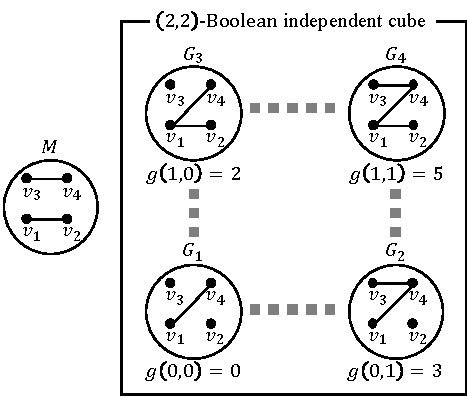
\includegraphics[width=0.88\linewidth]{fig/BoolCube.pdf}
  \vspace{-4mm}
  \caption{
    $(2,2)$-Boolean independent cube for $g$ corresponding to the $(4,2)$-independent cube for $f$ in Figure~\ref{chap1-fig:mono-cube}.
  }\label{chap1-fig:Bool-cube}
\end{figure}

Now, for $i \in [\kappa]$, define $\calS_i(x_i)$ for $x_i \in \{0,1\}$ by
% \[
\begin{align}
  \calS_i(x_i) = (\calR_{2i-1}(\bma_{2i-1} + x_i \bme_{2i}),
  \calR_{2i}(\bma_{2i} + x_i \bme_{2i-1})).
  \label{chap1-eq:S_i_R_2i_1}
\end{align}
% \]
In other words, $\calS_i(x_i)$ is simply the product of the outputs of users
$(v_{2i-1}, v_{2i})$, with $x_i$ indicating whether to add the edge in $M$ between them.

Assume that each $\calR_i$ is mutually independent and that $(\calR_1, \ldots, \calR_n)$ provides $\epsilon$-relationship DP in Definition~\ref{chap1-def:entire_edge_LDP}. 
Then by (\ref{chap1-eq:entire_edge_LDP}) and (\ref{chap1-eq:S_i_R_2i_1}), each $\calS_i$ provides $\epsilon$-DP and is mutually independent.
% Because the $\calR_i$ are mutually independent, we can conclude from
% Definition~\ref{chap1-def:entire_edge_LDP} that each $\calS_j(x)$ satisfies $\epsilon$-DP on the domain $\{0,1\}$. 

Define the estimator $\hat{g}$ by
\begin{align*}
  \hat{g}(x_1, \ldots, x_\kappa) &= \tilde{f}(\calS_1(x_1), \ldots,
  \calS_\kappa(x_\kappa)).
\end{align*}
Then by 
% We can apply 
Theorem~\ref{chap1-thm:lower-bound-dir}, 
% on $g$, $\hat{g}$, and the collection $\calS_1,\ldots, \calS_k$ to conclude that, 
for 
% $X \sim \{0,1\}^\kappa$,
$X=(x_1, \ldots, x_\kappa)$, 
\[
  \E_{X,\calS_1, \ldots, \calS_\kappa}[l_2^2(g(X), \hat{g}(X) )] \geq \Omega \left(
  \frac{e^{\varepsilon}}{(e^{\varepsilon}+1)^2} \kappa D^2 \right).
\]

Since 
% We are done by observing that 
there is a one-to-one correspondence between the ($n,D$)-independent cube $\calA$ 
and 
the ($\kappa,D$)-Boolean independent cube $\{0,1\}^\kappa$, we also have 
\[
  \E_{G,\calR_1, \ldots, \calR_n}[l_2^2(f(G), \hf(G))] \geq \Omega \left(
  \frac{e^{\varepsilon}}{(e^{\varepsilon}+1)^2} n D^2 \right),
\]
where $G$ is drawn uniformly from $\calA$, which proves Theorem~\ref{chap1-thm:lower-bound}. \qed
% and $\E_{\bmA, \calR_1, \ldots,
% \calR_n}[l_2^2(f(\bmA), \hf(\bmA))]$ is describing the same random process as
% $\E_{X, \calS_1, \ldots, \calS_k}[l_2^2(g(X), \hat{g}(X) )]$ with the variables
% renamed.

\subsection{Proof of
Theorem~\ref{chap1-thm:lower-bound-dir}}
\label{chap1-sub:proof_thm_lower-bound-dir}

Assume that $\calS_i : \{0,1\} \rightarrow \mathcal{Z}_i$.
For 
% $X \in \calX^n$, 
$X = (x_1, \ldots, x_\kappa) \in \{0,1\}^\kappa$, 
let $S(X) = (\calS_1(x_1), \cdots \calS_\kappa(x_\kappa))$ and
$Z = (z_1, \ldots, z_\kappa)$ with $z_i \in \mathcal{Z}_i$. 
We rewrite the quantity of interest as
\[
%\begin{align}
  \E_{X, S(X)}[l_2^2(g(X), \hg(X))] = \E_{X, S(X)}[(g(X)- \tilde{g}(S(X)))^2].
%  \label{chap1-eq:E_X_SX_l2}
\]
%\end{align}

% Using the law of total expectation, we condition on the event $S(X) = Z$:
By the law of total expectation, this quantity is the same as the expected value of the conditional expected value of $(g(X)- \tilde{g}(S(X)))^2$ given 
% we condition on the event 
$S(X) = Z$:
\begin{align}
  &\E_{X, S(X)}[(g(X)- \tilde{g}(S(X)))^2] \nonumber\\
  &= \E_{S(X)} \E_X[(g(X) - \tilde{g}(Z) )^2 | S(X)=Z].
  \label{chap1-eq:E_SX_X_g_tg}
\end{align}
% where for $Y \in \reals$
% $\E_{S(X)}[Y]$ represents the expectation of $Y$ over the randomness in $S$, and $\E_X[Y|S(X)=Z]$ represents the expectation of $Y$ over the randomness in selecting $X$ given $S(X)=Z$. 
Let $\mu_Z = \E_X[g(X)|S(X)=Z]$. 
Then the inner expectation in (\ref{chap1-eq:E_SX_X_g_tg}) can be written as follows:
% , with $\mu_Z = \E[g(X|S(X)=Z)]$,
\begin{align*}
  &\; \E_X[(g(X) - \tilde{g}(Z) )^2 | S(X)=Z] \\
  &= \E_X[( (g(X) - \mu_Z) + (\mu_Z - \tilde{g}(Z)) )^2 | S(X)=Z] \\
  &= \E_X[(g(X) - \mu_Z)^2 |S(X)=Z] \\
  &\hspace{3.5mm}+ 2(\mu_Z - \tilde{g}(Z))\E_X[(g(X) - \mu_Z)|S(X)=Z] \\
  &\hspace{3.5mm}+ (\mu_Z - \tilde{g}(Z))^2 \\
  &= \E_X[(g(X) - \mu_Z)^2 |S(X)=Z] + (\mu_Z - \tilde{g}(Z))^2 \\
  &= \V_X[g(X)|S(X)=Z] + (\mu_Z - \tilde{g}(Z))^2.
\end{align*}
Thus, it suffices to show that $\V_X[g(X)|S(X)=Z] \geq
\Omega\left(\frac{e^\epsilon}{(1+e^\epsilon)^2} \kappa D^2 \right)$.
For $B = (b_1, \ldots, b_\kappa) \in \{0,1\}^\kappa$, we have
\begin{align*}
  \Pr[X=B|S(X)=Z] = \frac{\Pr[X=B]\Pr[S(X)=Z|X=B]}{\Pr[S(X)=Z]}.
%   \Pr[X=B|S(X)=Z] &\propto \Pr[S(X)=Z|X=B]
\end{align*}
Since $\Pr[S(X)=Z]$ does not depend on $B$ and
$\Pr[X=B] = \frac{1}{2^\kappa}$, $\Pr[X=B|S(X)=Z]$ can also be expressed as 
\begin{align}
  \Pr[X=B|S(X)=Z] &\propto \Pr[S(X)=Z|X=B].
  \label{chap1-eq:X_B_SX_Z_propto}
\end{align}
% where the second line follows because $\Pr[S(X)=Z]$ does not depend on $B$ and
% $\Pr[X=B] = \frac{1}{2^\kappa}$.
% However, due to independence, 
Since $S_1, \ldots, S_\kappa$ are independently run, we have
% $\Pr[S(X)=Z|X=B]$ has the form
\begin{align*}
  \Pr[S(X)=Z|X=B] 
  &=
  %\;
  \Pr[\calS_1(b_1) = z_1, \ldots, \calS_\kappa(b_\kappa) = z_\kappa] \\
  &= \prod_{i=1}^\kappa \Pr[\calS_i(b_i)=z_i].
\end{align*}
Define 
%  \[
\begin{align*}
    % p_i = \frac{\Pr[\calS_i(x_i^{1})=z_i]}{\Pr[\calS_i(x_i^0)=z_i] +
    % \Pr[\calS_i(x_i^1)=z_i]}.
    p_i = \frac{\Pr[\calS_i(1)=z_i]}{\Pr[\calS_i(0)=z_i] +
    \Pr[\calS_i(1)=z_i]}.
%  \]
\end{align*}
Because each $\calS_i$ satisfies $\epsilon$-DP, we have $\frac{1}{1+e^{\epsilon}} \leq p_i \leq \frac{e^\epsilon}{1+e^\epsilon}$.
%The above equations tell us that
By (\ref{chap1-eq:X_B_SX_Z_propto}) and $\sum_{B \in \{0,1\}^\kappa} \Pr[X=B|S(X)=Z] = 1$, 
%$\Pr[X=B|S(X)=Z]$ can be expressed as 
we have
%  \[
\begin{align}
    \Pr[X=B|S(X)=Z] 
    %\propto 
    = 
    \prod_{i=1}^\kappa (p_i)^{b_i}(1-p_i)^{1-b_i}. %\\
%    &= \prod_{i=1}^\kappa \text{Bernoulli}(p_i),
%  \]
\label{chap1-eq:Pr_X_B_SX_Z_Bernoulli}
\end{align}
%where $\text{Bernoulli}(p_i)$ represents the Bernoulli distribution with parameter $p_i$.
This means that $\Pr[X=B|S(X)=Z]$ is distributed according to the independent product of $Bernoulli(p_i)$ for $i \in [\kappa]$.

Now, because 
%there is 
$g$ has 
a Boolean $(\kappa,D)$-independent cube, 
%for $g$, 
there are $C_1,
\ldots, C_\kappa \in \calS$ with $|C_i| \geq D$ such that
\begin{align*}
% g(X | S(X)=Z) &= g(0, \ldots, 0) + \sum_{i=1}^\kappa
% (x_i|S(X)=Z)C_i
g(X) &= g(0, \ldots, 0) + \sum_{i=1}^\kappa
x_iC_i.
\end{align*}
By (\ref{chap1-eq:Pr_X_B_SX_Z_Bernoulli}), 
% Because 
%$(x_i|S(X)=Z)$ 
$x_i$ 
is an independent draw from $Bernoulli(p_i)$ 
given $S(X)=Z$. 
Thus, the variance of 
%this quantity 
$g(X)$ given $S(X)=Z$ 
is
\begin{align*}
\V_X[g(X)|S(X)=Z] &= \sum_{i=1}^\kappa \V[x_i |S(X)=Z]C_i^2 \\
&\geq \sum_{i=1}^\kappa p_i(1-p_i) D^2 \\
&\geq \sum_{i=1}^\kappa \frac{e^\epsilon}{(1+e^\epsilon)^2} D^2 \\
&\geq \kappa \frac{e^\epsilon}{(1+e^\epsilon)^2} D^2.
\end{align*}
\qed
}
% \end{document}
